\documentclass[]{IEEEtran}
% some very useful LaTeX packages include:
%\usepackage{cite}      
\usepackage{graphicx}   
\usepackage{subfigure} 
\usepackage{url}       
\usepackage{amsmath}    
\usepackage{caption2}
% Your document starts here!
\begin{document}

% Define document title and author
	\title{Weekly Report}
	\author{Adviser: Prof. Yang Wen \\Student: Cheng Wensheng\\ Period: 2018.8.27-9.2
	}
	\markboth{Visual Information Processing Group}{}
	\maketitle

% Write abstract here
\begin{abstract}
	This week I mainly put my effort on improving deep learning methods accuracy of building extraction and writing the company project application.
\end{abstract}

% Each section begins with a \section{title} command
\section{Sar contest}
	% \PARstart{}{} creates a tall first letter for this first paragraph
	\PARstart{L}{ast} week we tried deep learning models and post-processing methods. This week, I found that the main error may come from false positive, which reduces the precision.
	\begin{itemize}
		\item I tried to change the division of training set and validation set. Since the 10th picture contains many objects which are bright and don't belong to buildings, I add this picture to training set. The result shows about 0.5$\%$ improvement, which means this is effective.
		\item To get more samples, I tried the python package Augmentor. I got reduced F1 score, which was weired. This week, I checked this again and found that the reason is I didn't pair original images and ground truth images. So I corrected this and uploaded it as the second chance this week.
	\end{itemize}
	
	Fig.~\ref{fig:fw} is neural network result. Fig.~\ref{fig:rt} is the ground truth image.


\section{Project application}
% \PARstart{}{} creates a tall first letter for this first paragraph
\PARstart{T}{his} week Zhang Heng, Yu Huai and I continued to improve the company project application. 
\begin{itemize}
	\item At first, we were supposed to write a brief version of the project application. Since Yu Huai went home, Zhang Heng and I revised his part and finished the four modules.
	\item On the weekend, Zhang Heng and I wrote the technical routine and implementation plan. We modified original content and drawed flowcharts with Microsoft Visio. Then I handed this to Mr.Lu.
	
\end{itemize}


% Main Part


\newpage


\begin{figure}
	\vspace{0.5cm}
%	\begin{minipage}[t]{0.5\linewidth}
		\centering
		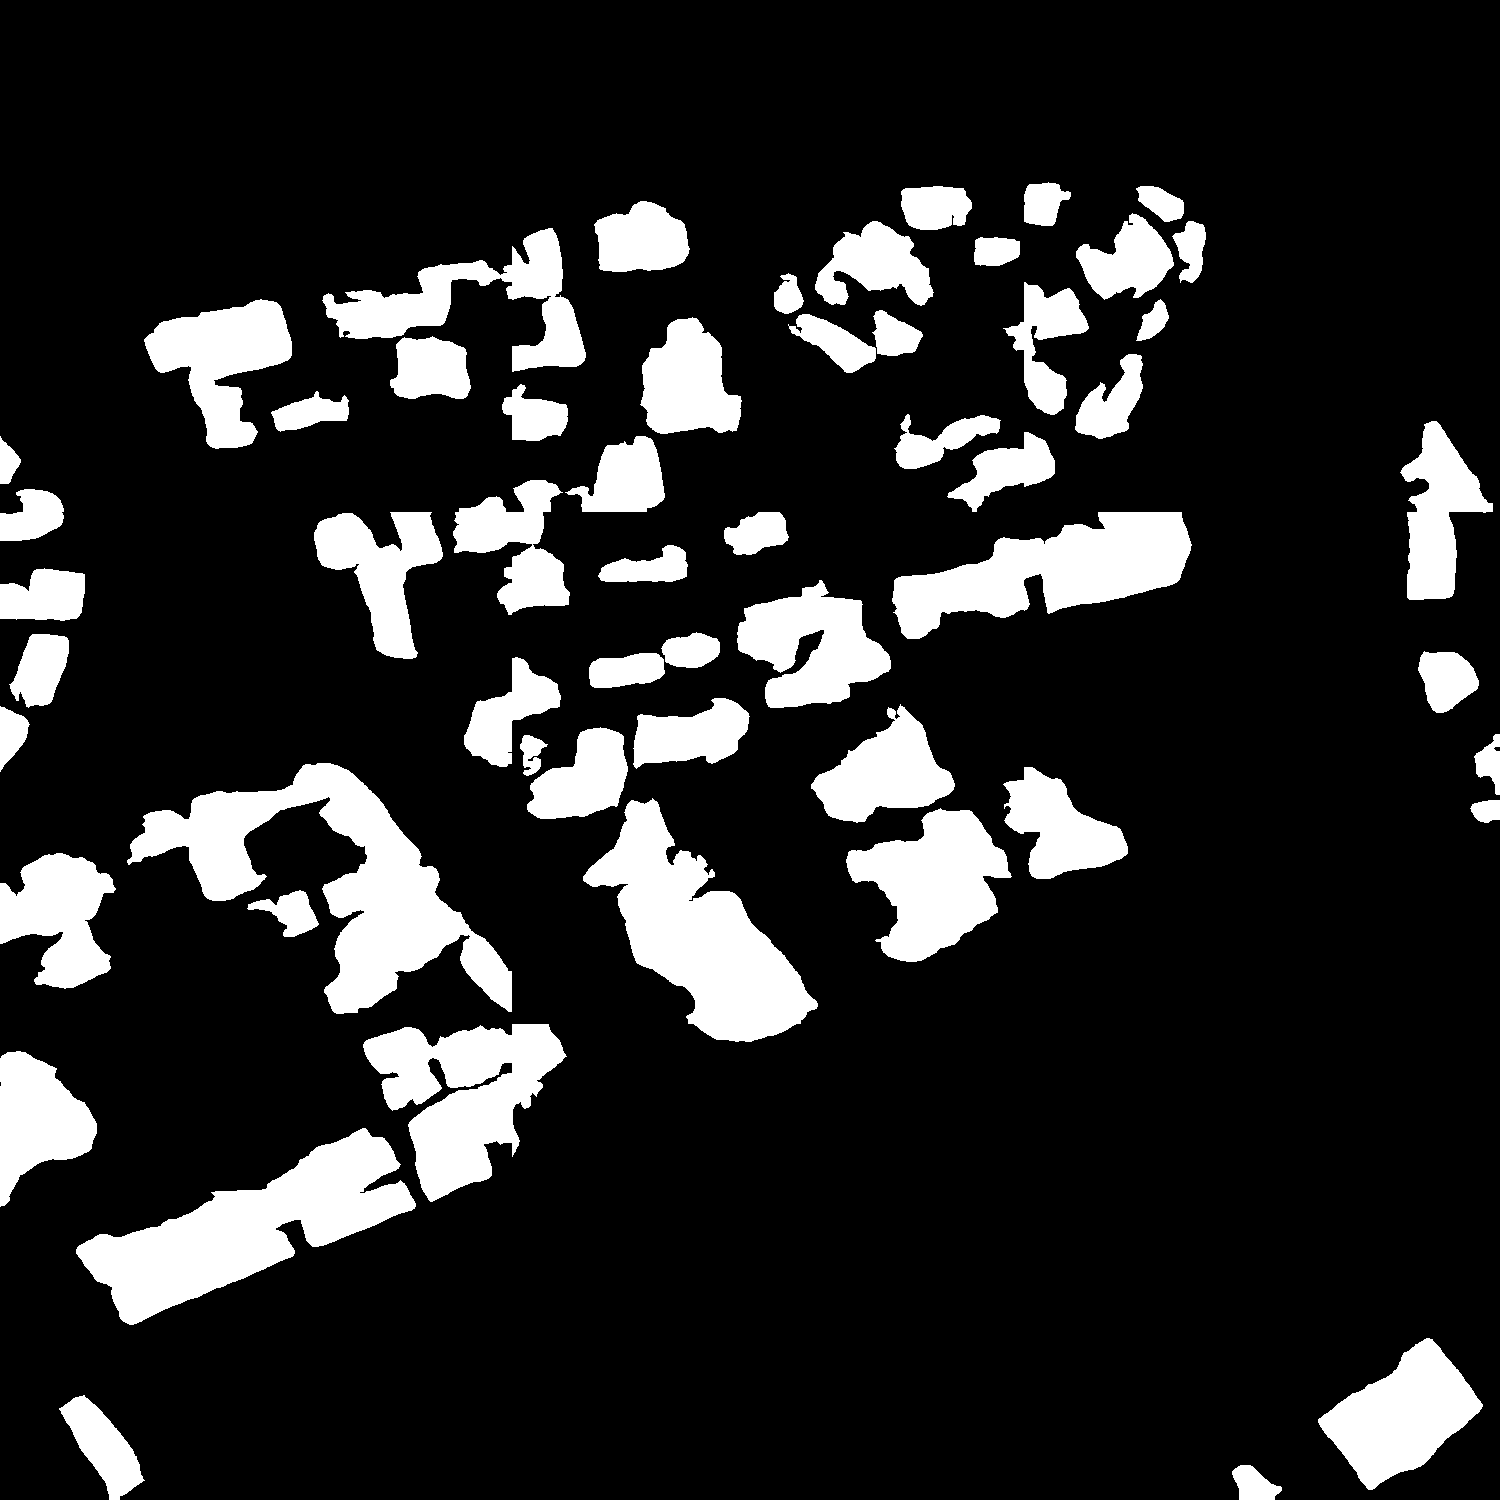
\includegraphics[width=0.7\columnwidth]{fw}
		\caption{Output result}
		\label{fig:fw}
%	\end{minipage}%
%	\begin{minipage}[t]{0.5\linewidth}
	\vspace{0.3cm}
		\centering
		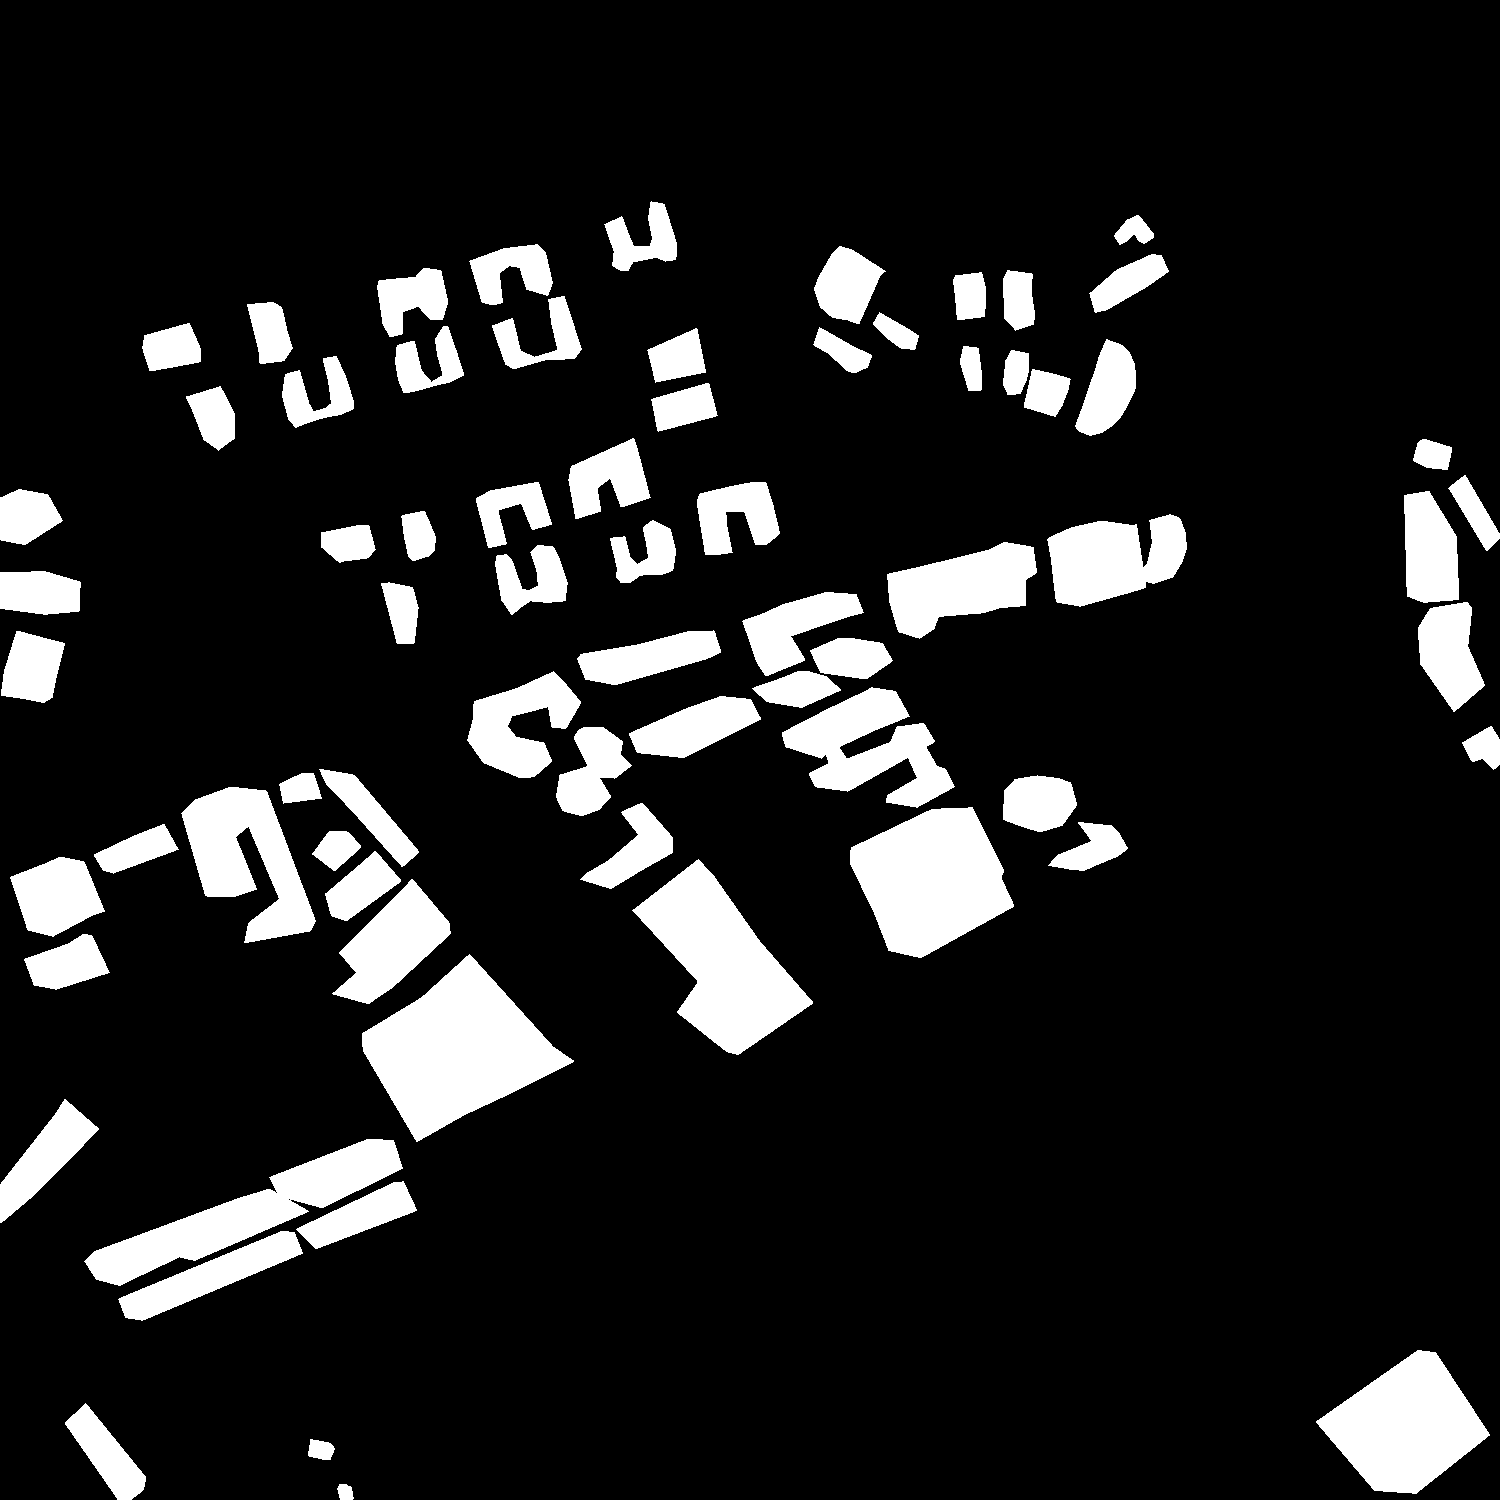
\includegraphics[width=0.7\columnwidth]{rt}
		\caption{Ground Truth}
		\label{fig:rt}
%	\end{minipage}
\end{figure}


%\begin{figure}[!hbt]
%%		 Center the figure.
%		\vspace{0.7cm}
%%		\hspace{50cm}
%		\begin{center}
%			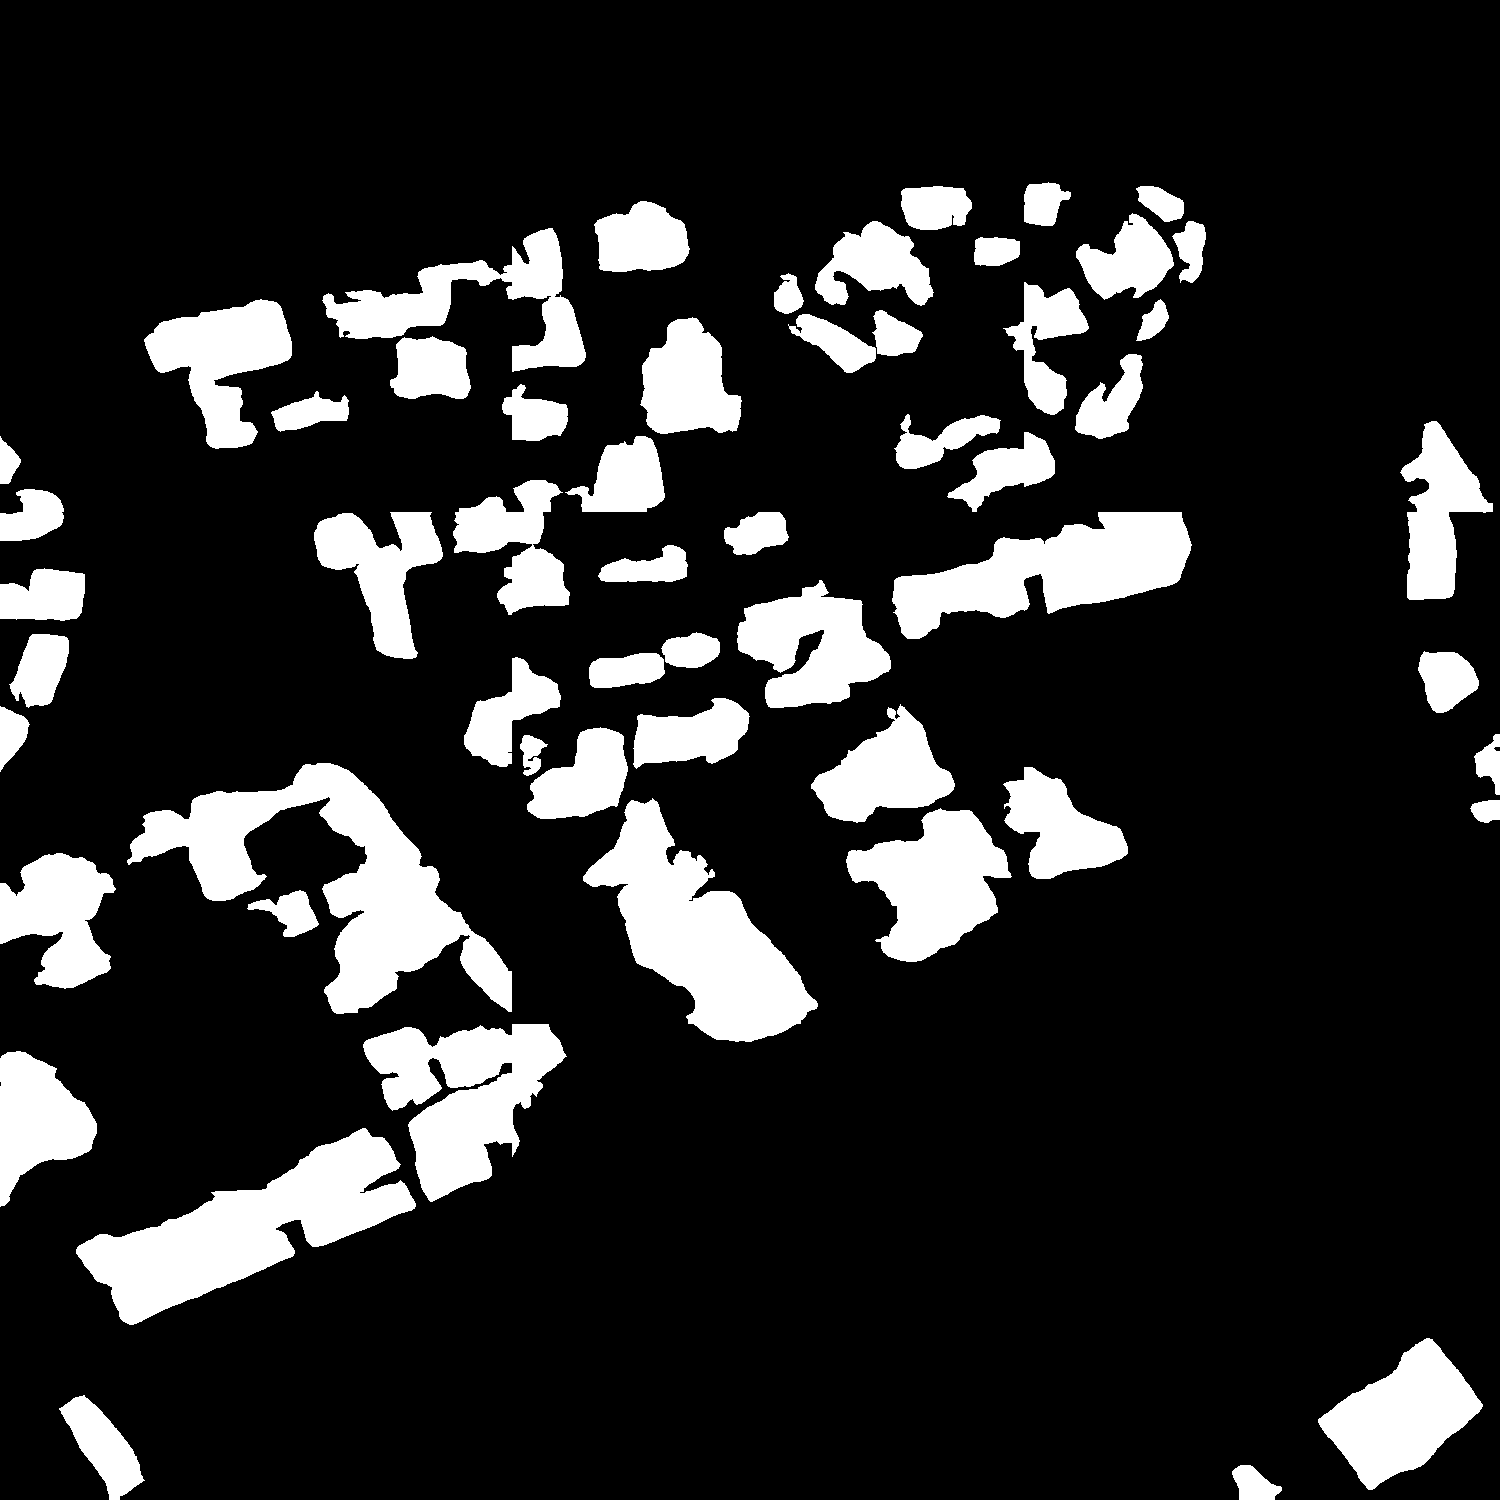
\includegraphics[width=0.2\columnwidth]{fw}
%				%		 Create a subtitle for the figure.
%			\caption{CNN methods result}
%			\label{fig:fw}
%		    \vspace{0.2cm}
%			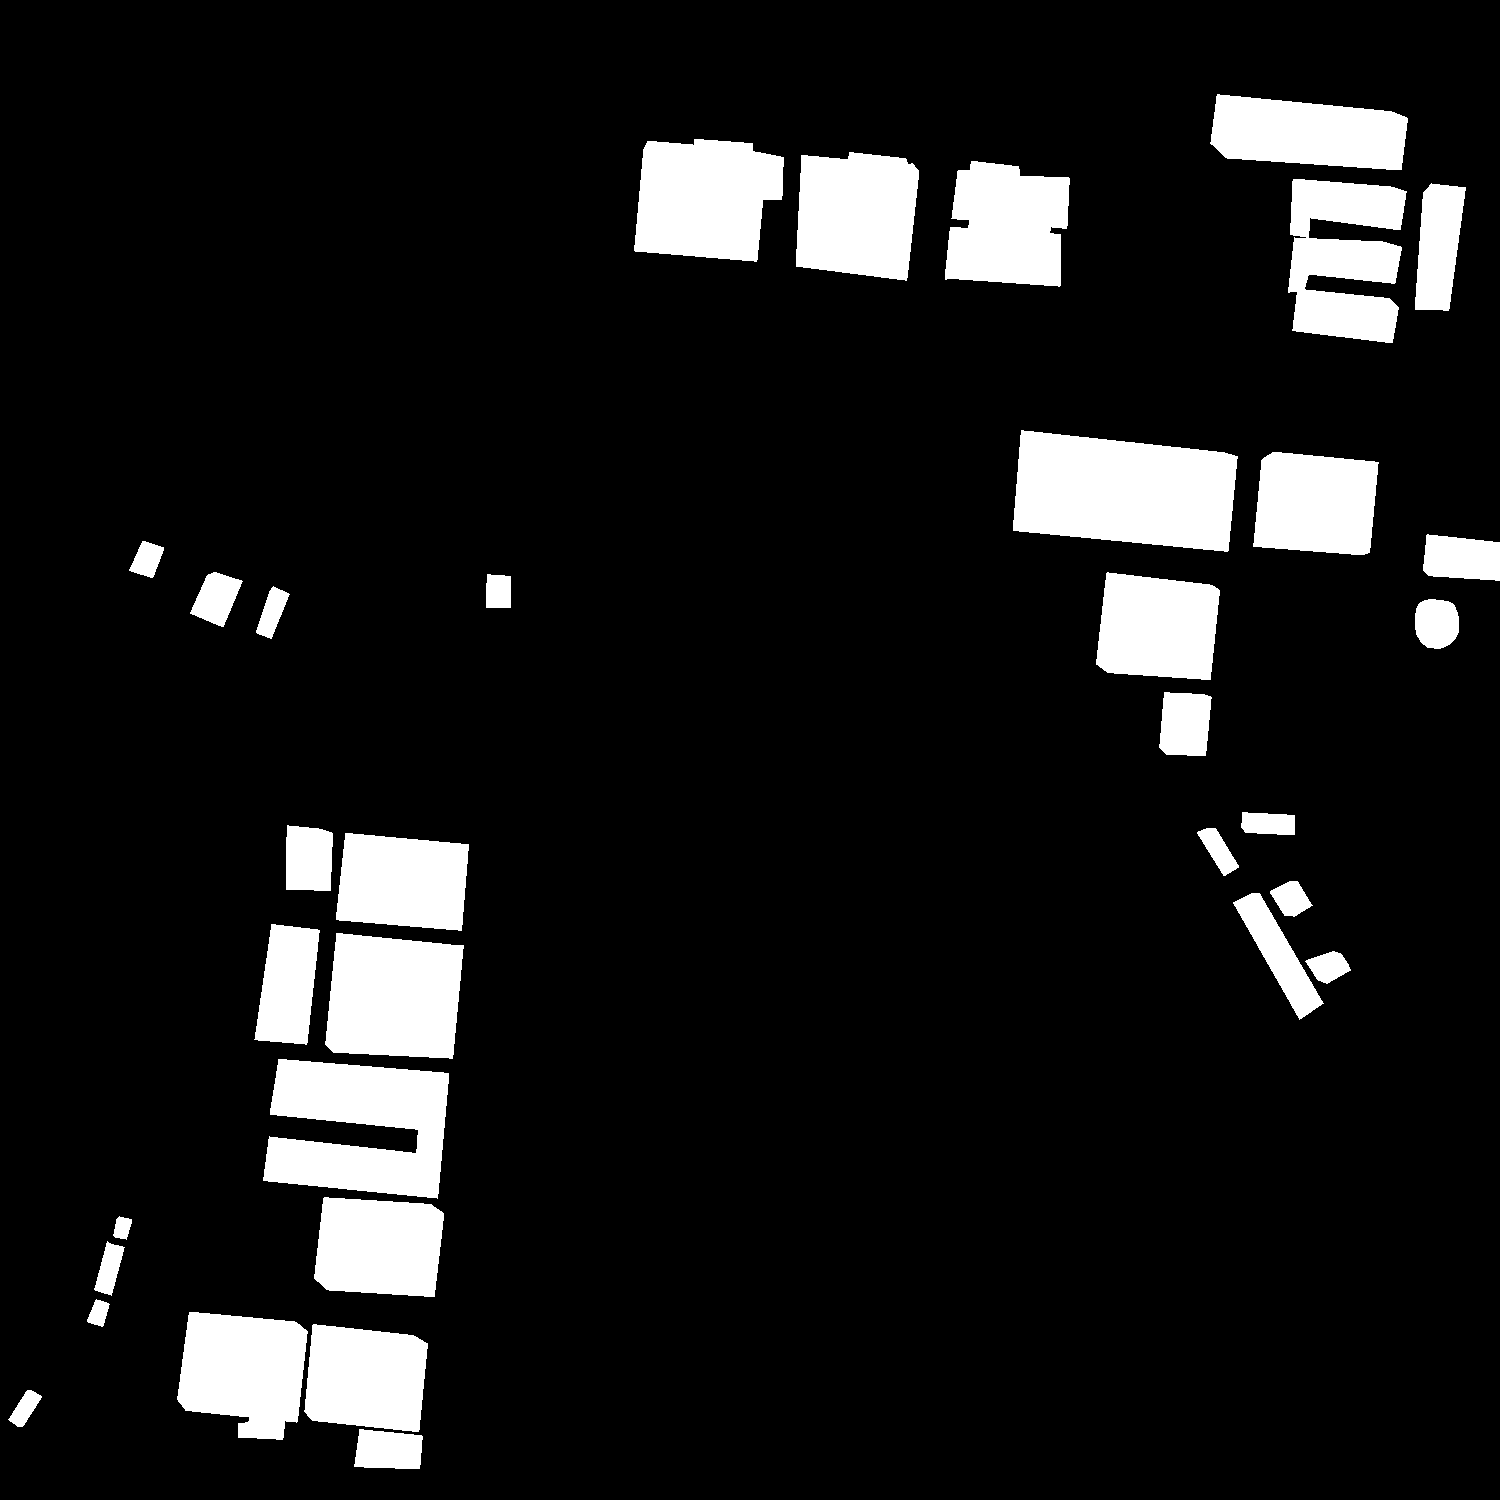
\includegraphics[width=0.2\columnwidth]{rs}
%				%Create a subtitle for the figure.
%			\caption{Ground truth}
%			\label{fig:rt}
%		\end{center}
%	\end{figure}



% Your document ends here!
\end{document}